% Options for packages loaded elsewhere
\PassOptionsToPackage{unicode}{hyperref}
\PassOptionsToPackage{hyphens}{url}
\PassOptionsToPackage{dvipsnames,svgnames,x11names}{xcolor}
%
\documentclass[
]{article}

\usepackage{amsmath,amssymb}
\usepackage{iftex}
\ifPDFTeX
  \usepackage[T1]{fontenc}
  \usepackage[utf8]{inputenc}
  \usepackage{textcomp} % provide euro and other symbols
\else % if luatex or xetex
  \usepackage{unicode-math}
  \defaultfontfeatures{Scale=MatchLowercase}
  \defaultfontfeatures[\rmfamily]{Ligatures=TeX,Scale=1}
\fi
\usepackage{lmodern}
\ifPDFTeX\else  
    % xetex/luatex font selection
  \setmainfont[]{Latin Modern Roman}
  \setmathfont[]{Latin Modern Math}
\fi
% Use upquote if available, for straight quotes in verbatim environments
\IfFileExists{upquote.sty}{\usepackage{upquote}}{}
\IfFileExists{microtype.sty}{% use microtype if available
  \usepackage[]{microtype}
  \UseMicrotypeSet[protrusion]{basicmath} % disable protrusion for tt fonts
}{}
\makeatletter
\@ifundefined{KOMAClassName}{% if non-KOMA class
  \IfFileExists{parskip.sty}{%
    \usepackage{parskip}
  }{% else
    \setlength{\parindent}{0pt}
    \setlength{\parskip}{6pt plus 2pt minus 1pt}}
}{% if KOMA class
  \KOMAoptions{parskip=half}}
\makeatother
\usepackage{xcolor}
\setlength{\emergencystretch}{3em} % prevent overfull lines
\setcounter{secnumdepth}{5}
% Make \paragraph and \subparagraph free-standing
\ifx\paragraph\undefined\else
  \let\oldparagraph\paragraph
  \renewcommand{\paragraph}[1]{\oldparagraph{#1}\mbox{}}
\fi
\ifx\subparagraph\undefined\else
  \let\oldsubparagraph\subparagraph
  \renewcommand{\subparagraph}[1]{\oldsubparagraph{#1}\mbox{}}
\fi


\providecommand{\tightlist}{%
  \setlength{\itemsep}{0pt}\setlength{\parskip}{0pt}}\usepackage{longtable,booktabs,array}
\usepackage{calc} % for calculating minipage widths
% Correct order of tables after \paragraph or \subparagraph
\usepackage{etoolbox}
\makeatletter
\patchcmd\longtable{\par}{\if@noskipsec\mbox{}\fi\par}{}{}
\makeatother
% Allow footnotes in longtable head/foot
\IfFileExists{footnotehyper.sty}{\usepackage{footnotehyper}}{\usepackage{footnote}}
\makesavenoteenv{longtable}
\usepackage{graphicx}
\makeatletter
\def\maxwidth{\ifdim\Gin@nat@width>\linewidth\linewidth\else\Gin@nat@width\fi}
\def\maxheight{\ifdim\Gin@nat@height>\textheight\textheight\else\Gin@nat@height\fi}
\makeatother
% Scale images if necessary, so that they will not overflow the page
% margins by default, and it is still possible to overwrite the defaults
% using explicit options in \includegraphics[width, height, ...]{}
\setkeys{Gin}{width=\maxwidth,height=\maxheight,keepaspectratio}
% Set default figure placement to htbp
\makeatletter
\def\fps@figure{htbp}
\makeatother
% definitions for citeproc citations
\NewDocumentCommand\citeproctext{}{}
\NewDocumentCommand\citeproc{mm}{%
  \begingroup\def\citeproctext{#2}\cite{#1}\endgroup}
\makeatletter
 % allow citations to break across lines
 \let\@cite@ofmt\@firstofone
 % avoid brackets around text for \cite:
 \def\@biblabel#1{}
 \def\@cite#1#2{{#1\if@tempswa , #2\fi}}
\makeatother
\newlength{\cslhangindent}
\setlength{\cslhangindent}{1.5em}
\newlength{\csllabelwidth}
\setlength{\csllabelwidth}{3em}
\newenvironment{CSLReferences}[2] % #1 hanging-indent, #2 entry-spacing
 {\begin{list}{}{%
  \setlength{\itemindent}{0pt}
  \setlength{\leftmargin}{0pt}
  \setlength{\parsep}{0pt}
  % turn on hanging indent if param 1 is 1
  \ifodd #1
   \setlength{\leftmargin}{\cslhangindent}
   \setlength{\itemindent}{-1\cslhangindent}
  \fi
  % set entry spacing
  \setlength{\itemsep}{#2\baselineskip}}}
 {\end{list}}
\usepackage{calc}
\newcommand{\CSLBlock}[1]{\hfill\break\parbox[t]{\linewidth}{\strut\ignorespaces#1\strut}}
\newcommand{\CSLLeftMargin}[1]{\parbox[t]{\csllabelwidth}{\strut#1\strut}}
\newcommand{\CSLRightInline}[1]{\parbox[t]{\linewidth - \csllabelwidth}{\strut#1\strut}}
\newcommand{\CSLIndent}[1]{\hspace{\cslhangindent}#1}

\usepackage{arxiv}
\usepackage{orcidlink}
\usepackage{amsmath}
\usepackage[T1]{fontenc}
\makeatletter
\@ifpackageloaded{caption}{}{\usepackage{caption}}
\AtBeginDocument{%
\ifdefined\contentsname
  \renewcommand*\contentsname{Table of contents}
\else
  \newcommand\contentsname{Table of contents}
\fi
\ifdefined\listfigurename
  \renewcommand*\listfigurename{List of Figures}
\else
  \newcommand\listfigurename{List of Figures}
\fi
\ifdefined\listtablename
  \renewcommand*\listtablename{List of Tables}
\else
  \newcommand\listtablename{List of Tables}
\fi
\ifdefined\figurename
  \renewcommand*\figurename{Figure}
\else
  \newcommand\figurename{Figure}
\fi
\ifdefined\tablename
  \renewcommand*\tablename{Table}
\else
  \newcommand\tablename{Table}
\fi
}
\@ifpackageloaded{float}{}{\usepackage{float}}
\floatstyle{ruled}
\@ifundefined{c@chapter}{\newfloat{codelisting}{h}{lop}}{\newfloat{codelisting}{h}{lop}[chapter]}
\floatname{codelisting}{Listing}
\newcommand*\listoflistings{\listof{codelisting}{List of Listings}}
\makeatother
\makeatletter
\makeatother
\makeatletter
\@ifpackageloaded{caption}{}{\usepackage{caption}}
\@ifpackageloaded{subcaption}{}{\usepackage{subcaption}}
\makeatother
\ifLuaTeX
  \usepackage{selnolig}  % disable illegal ligatures
\fi
\usepackage{bookmark}

\IfFileExists{xurl.sty}{\usepackage{xurl}}{} % add URL line breaks if available
\urlstyle{same} % disable monospaced font for URLs
\hypersetup{
  pdftitle={Spatial Modeling of Cardiovascular Disease Associated with Increasing Airborne Particulate Matter},
  pdfauthor={Johan Booc; Christina Kim; Shombit Roy},
  pdfkeywords={Fine Particulate Matter (PM2\_5), Cardiovascular Disease
(CVD), Cardiovascular Mortality (CVM)},
  colorlinks=true,
  linkcolor={blue},
  filecolor={Maroon},
  citecolor={Blue},
  urlcolor={Blue},
  pdfcreator={LaTeX via pandoc}}

\newcommand{\runninghead}{A Preprint }
\renewcommand{\runninghead}{CVD Related to PM2.5 }
\title{Spatial Modeling of Cardiovascular Disease Associated with
Increasing Airborne Particulate Matter}
\def\asep{\\\\\\ } % default: all authors on same column
\author{\textbf{Johan Booc}\\Department of Statistics\\Texas A\&M
University\\\\\href{mailto:jbooc24@tamu.edu}{jbooc24@tamu.edu}\asep\textbf{Christina
Kim}\\Department of Statistics\\Texas A\&M
University\\\\\href{mailto:christinaykim3@tamu.edu}{christinaykim3@tamu.edu}\asep\textbf{Shombit
Roy}\\Department of Statistics\\Texas A\&M
University\\\\\href{mailto:shombit123@tamu.edu}{shombit123@tamu.edu}}
\date{}
\begin{document}
\maketitle
\begin{abstract}
Cardiovascular disease (CVD) stands as the leading cause of death in the
United States. By using spatial modeling techniques, such as
geographically weighted regression (GWR), we have determined that CVD
will see an increasing incidence rate outside the Stroke Belt region as
the concentration of air pollutants increases and socioeconomic factors
worsen. Policymakers and health practice practitioners are thus able to
use these results in justifying targeted interventions to curb the
increasing rates of CVD, aiming to halt one of the world's deadliest
diseases.
\end{abstract}
{\bfseries \emph Keywords}
\def\sep{\textbullet\ }
Fine Particulate Matter (PM2\_5) \sep Cardiovascular Disease (CVD) \sep 
Cardiovascular Mortality (CVM)


\section{Introduction}\label{sec-intro}

\begin{itemize}
\item
  Broad strokes: Explain how cardiovascular disease is the leading cause
  of death in the US, our paper filing the gap by putting the focus on
  the 18-44-year-old age group~
\item
  Specifics: Explicitly state how the CVD incidence rate varies
  spatially in the US, for our covariates. Our approach involves
  analyzing this relationship to produce risk prediction estimates for
  our specified age group.~
\item
  Central thesis: Use a geographically weighted model approach to
  produce visualizations and analyze the relationship between our
  response variable (CVD deaths) and its covariates (air pollutant
  concentration and socioeconomic factors), specifically focusing on
  spatial variation.~
\item
  Step back: The overall outcome of our study involves aiding
  policymakers and health practitioners develop the necessary
  interventions in the targeted regions that are most affected by
  CVD.Related Works
\end{itemize}

Paragraph 1) Review of regression approaches in cardiovascular disease
mortality 2) Review of geographically weighted regression models 3) GWR
with CVD 4) Risk prediction Model 5) Direct comparison with clustering
approaches

\section{Related Works}\label{related-works}

\begin{enumerate}
\def\labelenumi{\arabic{enumi}.}
\item
  Review of regression approaches in cardiovascular disease mortality~
\item
  Review of geographically weighted regression models~
\item
  GWR with CVD~
\item
  Risk prediction model~
\item
  Direct comparison with clustering approaches
\end{enumerate}

\section{Methods}\label{methods}

\subsubsection{Data}\label{data}

\begin{itemize}
\item
  Combination of four data sets (will add citations later): CDC
  cardiovascular disease death rates per US counties, NASA particulate
  matter concentrations for the year 2015, US Census Data for 2015, and
  US Vaccination rate by county data

  \begin{itemize}
  \tightlist
  \item
    Vaccination rates were not considered in the study, rather, the
    dataset was used for its geometry listing, which will be important
    for our GWR section.
  \end{itemize}
\item
  We merged the four data sets together to analyze multiple variables
  against the CVM per 100,000 residents in each county. Variables
  included \% of race present in county, PM2.5 concentrations, median
  income, and unemployment rates.
\end{itemize}

\subsubsection{Geographically Weighted Regression
Model}\label{geographically-weighted-regression-model}

\begin{itemize}
\item
  Local Significance

  \begin{itemize}
  \item
    Coefficients have t-values and SE values, converted t-values into
    p-values with formula from code, extracted these p-values for each
    covariate and then plotted significance from p-values. The results
    of this should show which covariates have higher effects per county
  \item
    Per our (source), different regions of the United States should have
    different variables with greater significance relating to CVD rates.

    \begin{itemize}
    \tightlist
    \item
      For example, in the midwest, food insecurity was found to be the
      most significant factor, while in the West it did not play much of
      a role compared to income, PM2.5, and access to healthcare.
    \end{itemize}
  \end{itemize}
\end{itemize}

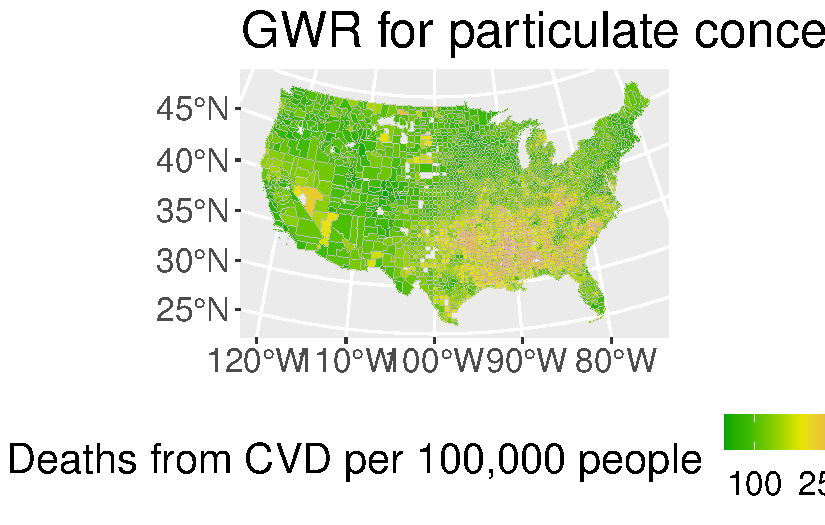
\includegraphics{report_files/figure-pdf/unnamed-chunk-2-1.pdf}

\section{Results}\label{results}

\begin{verbatim}
   ***********************************************************************
   *                       Package   GWmodel                             *
   ***********************************************************************
   Program starts at: 2024-04-10 16:00:56.459518 
   Call:
   gwr.basic(formula = Data_Vl ~ prc_wht + prc_frc + prc_hsp + perc_sn + 
    p2_5_20 + estimat + U__2015, data = mergedf_spatial, bw = opt_bandwidth, 
    kernel = "gaussian", adaptive = FALSE, parallel.method = "omp")

   Dependent (y) variable:  Data_Vl
   Independent variables:  prc_wht prc_frc prc_hsp perc_sn p2_5_20 estimat U__2015
   Number of data points: 3057
   ***********************************************************************
   *                    Results of Global Regression                     *
   ***********************************************************************

   Call:
    lm(formula = formula, data = data)

   Residuals:
     Min       1Q   Median       3Q      Max 
-133.061  -22.813   -5.661   19.637  202.340 

   Coefficients:
                 Estimate Std. Error t value Pr(>|t|)    
   (Intercept)  2.388e+02  1.024e+01  23.313  < 2e-16 ***
   prc_wht     -8.158e+01  9.500e+00  -8.587  < 2e-16 ***
   prc_frc      5.526e+01  9.988e+00   5.532 3.42e-08 ***
   prc_hsp     -9.321e+01  1.023e+01  -9.107  < 2e-16 ***
   perc_sn     -2.090e+02  3.425e+01  -6.101 1.18e-09 ***
   p2_5_20      6.311e+00  4.453e-01  14.170  < 2e-16 ***
   estimat     -2.120e-03  7.150e-05 -29.648  < 2e-16 ***
   U__2015      3.736e+00  4.118e-01   9.072  < 2e-16 ***

   ---Significance stars
   Signif. codes:  0 '***' 0.001 '**' 0.01 '*' 0.05 '.' 0.1 ' ' 1 
   Residual standard error: 35.64 on 3049 degrees of freedom
   Multiple R-squared: 0.6105
   Adjusted R-squared: 0.6096 
   F-statistic: 682.6 on 7 and 3049 DF,  p-value: < 2.2e-16 
   ***Extra Diagnostic information
   Residual sum of squares: 3873809
   Sigma(hat): 35.6093
   AIC:  30534.31
   AICc:  30534.37
   BIC:  27603.76
   ***********************************************************************
   *          Results of Geographically Weighted Regression              *
   ***********************************************************************

   *********************Model calibration information*********************
   Kernel function: gaussian 
   Fixed bandwidth: 128251.7 
   Regression points: the same locations as observations are used.
   Distance metric: Euclidean distance metric is used.

   ****************Summary of GWR coefficient estimates:******************
                    Min.     1st Qu.      Median     3rd Qu.      Max.
   Intercept -1.8237e+02  1.6625e+02  2.7812e+02  4.1353e+02 2293.3931
   prc_wht   -1.7708e+03 -2.3314e+02 -1.1902e+02 -3.3864e+01  309.4663
   prc_frc   -1.9197e+03 -2.0396e+02 -6.1895e+01  5.2242e+01 3229.3222
   prc_hsp   -1.7720e+03 -2.8864e+02 -1.5801e+02 -6.4279e+01  504.0406
   perc_sn   -1.9199e+03 -6.5045e+02 -3.4826e+02 -1.4864e+02 1635.4916
   p2_5_20   -4.8476e+01 -9.9089e-01  3.7131e+00  9.5388e+00   41.5626
   estimat   -8.0369e-03 -2.6333e-03 -1.8226e-03 -1.1243e-03    0.0017
   U__2015   -7.0110e+00  2.6200e+00  5.3167e+00  7.4156e+00   18.3070
   ************************Diagnostic information*************************
   Number of data points: 3057 
   Effective number of parameters (2trace(S) - trace(S'S)): 576.851 
   Effective degrees of freedom (n-2trace(S) + trace(S'S)): 2480.149 
   AICc (GWR book, Fotheringham, et al. 2002, p. 61, eq 2.33): 28146.12 
   AIC (GWR book, Fotheringham, et al. 2002,GWR p. 96, eq. 4.22): 27581.59 
   BIC (GWR book, Fotheringham, et al. 2002,GWR p. 61, eq. 2.34): 27506.99 
   Residual sum of squares: 1290938 
   R-square value:  0.8701873 
   Adjusted R-square value:  0.8399823 

   ***********************************************************************
   Program stops at: 2024-04-10 16:00:57.779456 
\end{verbatim}

Table Summary interpretation: The analysis compares two distinct
statistical models to explore the relationships between socio-economic,
demographic, and environmental variables and death rates. The first is a
global regression model which, despite revealing that all predictors are
highly statistically significant, does not take into account spatial
correlation. Hence, while the model does suggest that our variables are
indeed important, the global model may overlook local variations that
are crucial in understanding the true nature of the data.~

On the other hand, the geographically weighted regression (GWR) model
incorporates spatial variation, which is a critical factor given the
context of the data. We can see how well the GWR model worked by looking
at the R-squared value, which is .870, a significant improvement over
the global model. This R-squared value, along with the use of localized
spatial statistics, confirms the non-uniform relationship between the
predictors and the response variable across different geographical
areas. In summary, the GWR model, by accommodating the spatial component
present in the data, provides a more realistic interpretation of how
various factors influence death rates across different regions.

Significance plot:-~

The plots provided depict the local significance and magnitude of
different parameters (covariates) from a geographically weighted
regression (GWR) model, focusing on their relationship with death rates
across the United States. The areas in red indicate regions where the
covariates are statistically significant, and the color's intensity
represents the effect's magnitude.

\begin{figure}

\begin{minipage}{0.50\linewidth}
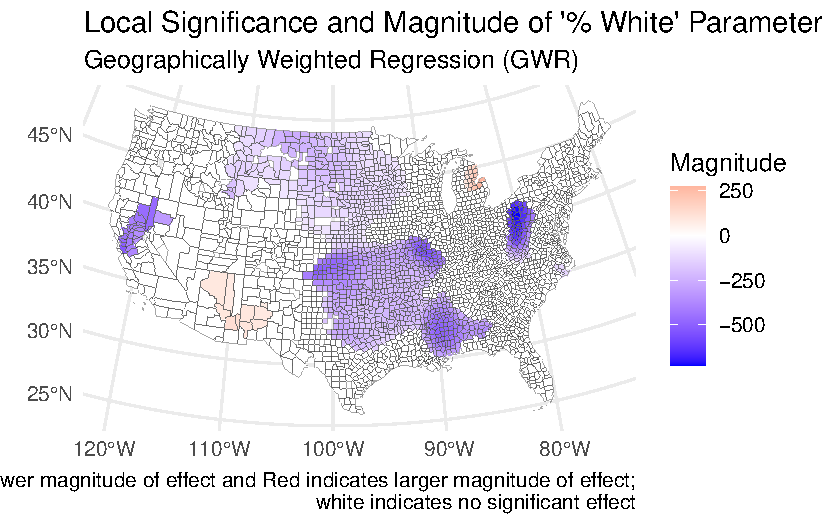
\includegraphics{report_files/figure-pdf/unnamed-chunk-4-1.pdf}\end{minipage}%
%
\begin{minipage}{0.50\linewidth}
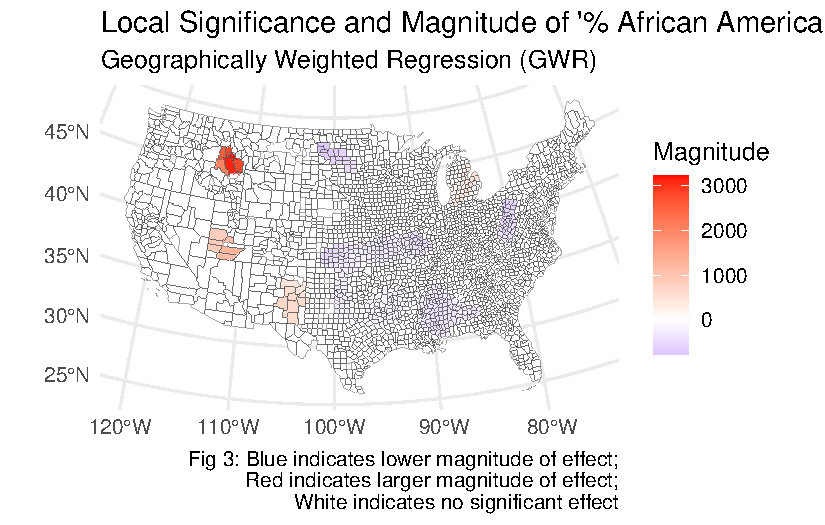
\includegraphics{report_files/figure-pdf/unnamed-chunk-4-2.pdf}\end{minipage}%
\newline
\begin{minipage}{0.50\linewidth}
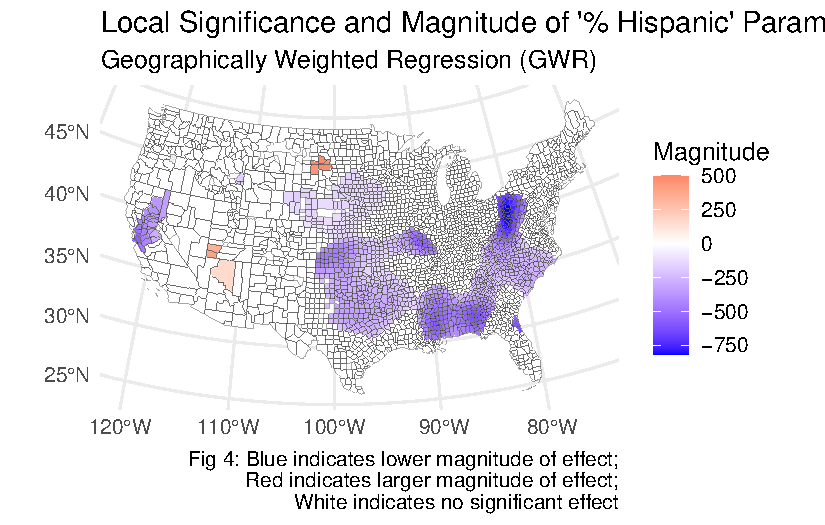
\includegraphics{report_files/figure-pdf/unnamed-chunk-4-3.pdf}\end{minipage}%
%
\begin{minipage}{0.50\linewidth}
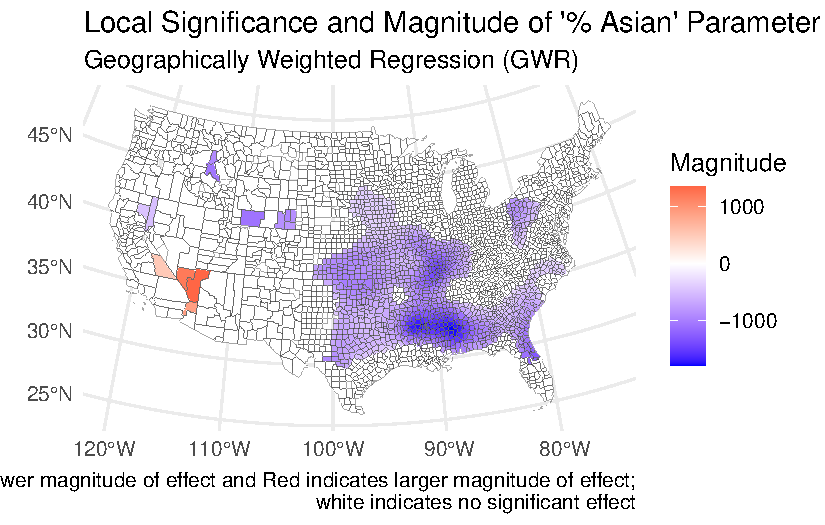
\includegraphics{report_files/figure-pdf/unnamed-chunk-4-4.pdf}\end{minipage}%

\end{figure}%

\begin{itemize}
\tightlist
\item
  Demographic Impact: The percentage of white and Hispanic populations
  shows significant regional variations in association with death rates.
  Higher proportions of white populations correlate with lower death
  rates in central areas, whereas higher percentages of Hispanic
  populations are linked to lower death rates in the West and Southwest.
  Conversely, higher percentages of African American populations are
  associated with higher death rates in certain Midwestern and
  Southeastern regions.
\end{itemize}

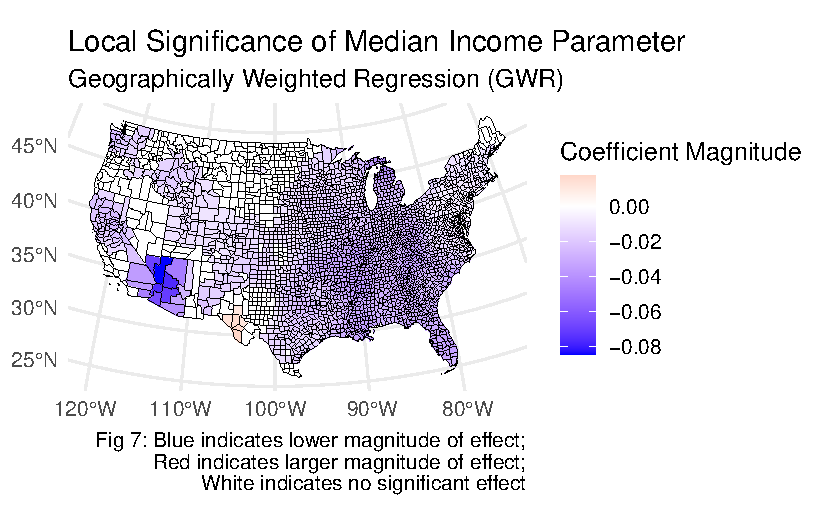
\includegraphics{report_files/figure-pdf/unnamed-chunk-5-1.pdf}

\begin{itemize}
\item
  Environmental Influence: Air quality, indicated by PM2.5 levels,
  demonstrates a significant positive relationship with death rates,
  particularly east of the Rockies, highlighting environmental health as
  a major concern.

  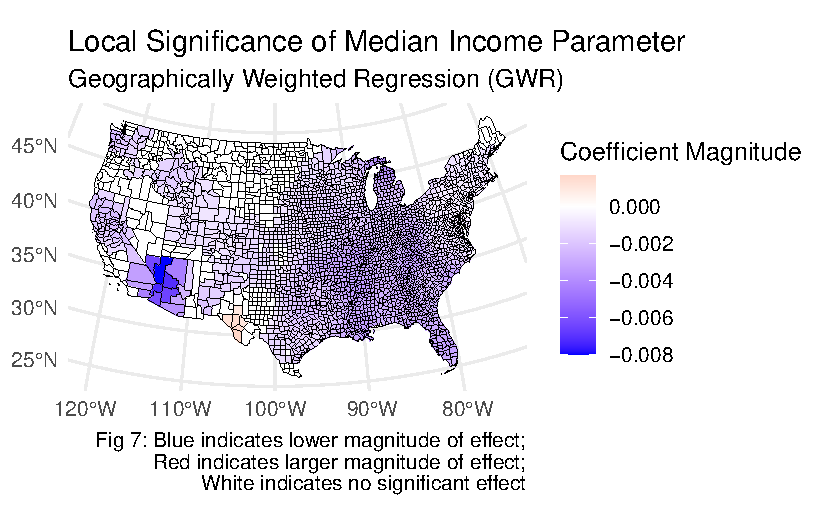
\includegraphics{report_files/figure-pdf/unnamed-chunk-6-1.pdf}

  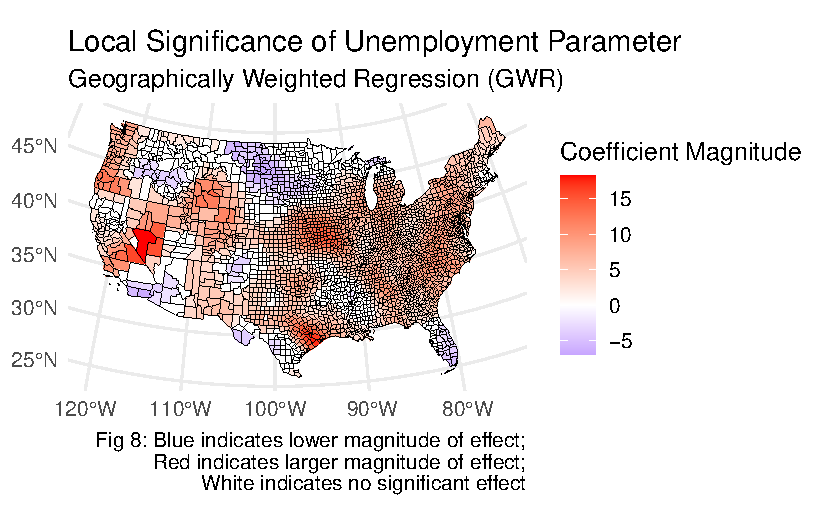
\includegraphics{report_files/figure-pdf/unnamed-chunk-6-2.pdf}
\end{itemize}

\begin{itemize}
\tightlist
\item
  Socio-economic Correlation: Median income levels across many regions
  show a consistent negative association with death rates, suggesting
  that higher income areas generally experience fewer deaths.
\end{itemize}

\section{Discussion}\label{discussion}

These maps reveal that the relationships between race, socio-economic
factors, environmental quality, and death rates are complex and highly
localized. The significance and strength of these relationships vary
considerably across different parts of the United States. For example,~

\begin{itemize}
\tightlist
\item
  Socio-economic factors like income show widespread significance,
  implying a consistent relationship with health outcomes across various
  locations.
\end{itemize}

\begin{itemize}
\tightlist
\item
  Race impacts are significant in certain areas, which may reflect
  underlying health disparities, access to care, or other social
  determinants of health.
\end{itemize}

\begin{itemize}
\tightlist
\item
  Air quality has a broad impact, suggesting environmental health
  concerns that might require region-specific policies.~
\end{itemize}

\newpage{}

\section*{References}\label{references}
\addcontentsline{toc}{section}{References}

\phantomsection\label{refs}
\begin{CSLReferences}{1}{0}
\bibitem[\citeproctext]{ref-article-journal}
n.d.

\end{CSLReferences}

(n.d.)



\end{document}
